% Created 2024-12-08 Sun 16:02
% Intended LaTeX compiler: pdflatex
\documentclass[letterpaper, 14pt]{article}
\usepackage[utf8]{inputenc}
\usepackage[T1]{fontenc}
\usepackage{graphicx}
\usepackage{longtable}
\usepackage{wrapfig}
\usepackage{rotating}
\usepackage[normalem]{ulem}
\usepackage{amsmath}
\usepackage{amssymb}
\usepackage{capt-of}
\usepackage{hyperref}
\usepackage{minted}
\usepackage{xcolor}
\usepackage{hyperref}
\usepackage{tocloft}
\usepackage{minted}
\usemintedstyle{manni}
\usepackage{pdfpages}
\usepackage{fancyhdr}
\usepackage{graphicx}
\usepackage[top=1.4in, left=0.5in, right=0.5in, bottom=0.8in]{geometry}
\usepackage[T1]{fontenc}
\usepackage{helvet}
\pagestyle{fancy}
\renewcommand{\headrulewidth}{0pt}
\renewcommand{\footrulewidth}{0pt}
\setlength{\parindent}{0em}
\setlength{\parskip}{1em}
\usepackage{hyperref}
\usepackage {color}
\usepackage {tabularray}
\usepackage{xcolor}
\hypersetup{
colorlinks=true,
linkcolor=blue,
filecolor=magenta,
urlcolor=cyan,
citecolor=green,
pdfborder={0 0 0}
}
\usepackage[most]{tcolorbox}
\author{Hilduara Abreu}
\date{2024-12-06}
\title{School Year 2024-25 | Principal Message December 2024}
\hypersetup{
 pdfauthor={Hilduara Abreu},
 pdftitle={School Year 2024-25 | Principal Message December 2024},
 pdfkeywords={},
 pdfsubject={},
 pdfcreator={Emacs 29.3 (Org mode 9.6.15)}, 
 pdflang={English}}
\begin{document}

\fancyfoot[C]{\setlength{\unitlength}{1in}\begin{picture}(5,0)\put(-1.8,-0.5){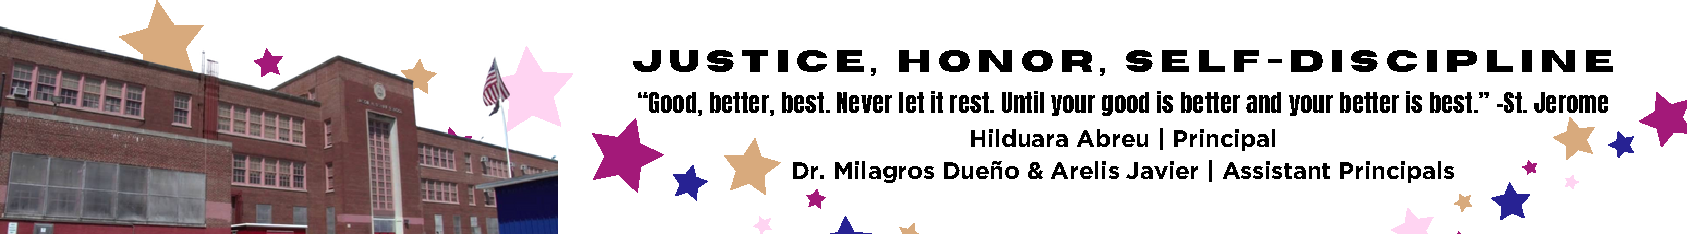
\includegraphics[width=8.8in,height=1.3in]{logo-1}}\end{picture}}
\fancyhead[C]{\setlength{\unitlength}{1in}\begin{picture}(5,0)\put(-1.9,-0.5){
\includegraphics[width=8.9in,height=1.3in]{logo-2}}\end{picture}}
\fancyhead[R]{\thepage}
\pagenumbering{gobble}

\begin{document}
\newpage
\vspace*{-0.2cm}
\emph{\textbf{Subject: Welcome to December, 2024 at PS 192: The School of Joyful Learning!}}

Dear PS192 Community,

As we approach the close of another year, we would like to extend our warmest wishes for a joyous and meaningful Holiday Season! It is hard to believe that we are already in December—just three short months since we opened our doors for the new school year. Reflecting on the time that has passed, our school has been buzzing with exciting events and enriching learning experiences that would take several pages to fully capture.

It was truly a pleasure to celebrate Thanksgiving with our wonderful students, and it was heartwarming to see parents and families join in the festivities. Your presence and engagement mean so much to our school community.

Looking ahead, we are excited to continue spreading the Holiday Spirit with our annual Holiday Breakfast. Please join us for this special celebration, as well as Coffee with the Principal, on Friday, December 20, at 8:00 a.m. in the Gym. It’s a wonderful opportunity to come together as a school family.

Additionally, we encourage parents to make time for instructional activities during the holiday break. Simple practices like engaging in math exercises, reading with your child, or encouraging independent reading and writing can make a significant impact. Creating a daily journal with your child is also a great way to capture and cherish the special moments you share over the holidays.

We are also thrilled to highlight our new initiative: "Reading at Home: Nurturing Infinite Potential through Literacy," which started last month. This program is designed to help parents support their child's literacy development at home. You can find valuable resources and guidance by visiting \href{https://www.ps192.org/reading-at-home}{Reading at Home}.

Each month, we will feature a Book of the Month. Check your child's grade-specific recommendations on the webpage for details. Additionally, we encourage you to utilize your child’s i-Ready account for more personalized learning resources, and explore a world of free literature through \href{https://www.ps192.org/project-gutenberg}{Project Gutenberg}. New resources are added each month to enhance your child’s learning journey.

On behalf of the PS 192 staff, we wish you a safe, happy, and fulfilling Holiday Season. Thank you for your continued partnership in fostering a vibrant, supportive, and engaged learning community.

With Justice, Honor, and Self-Discipline,


\includegraphics[width=0.2\textwidth]{hil_signature}

\textbf{Hilduara Abreu, Principal}

\textbf{The School of Joyful Learning!}

\href{www.ps192.org}{www.ps192.org}

\newpage

\fancyfoot[C]{\setlength{\unitlength}{1in}\begin{picture}(5,0)\put(-1.8,-0.5){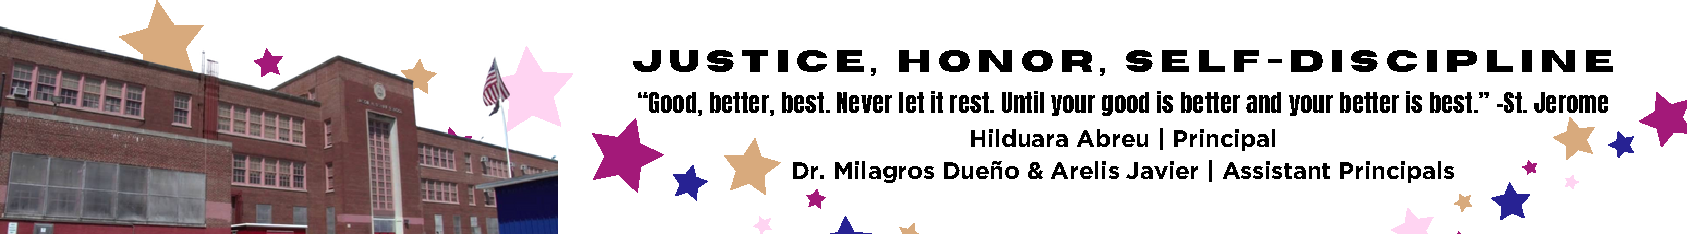
\includegraphics[width=8.8in,height=1.3in]{logo-1}}\end{picture}}
\fancyhead[C]{\setlength{\unitlength}{1in}\begin{picture}(5,0)\put(-1.9,-0.5){
\includegraphics[width=8.9in,height=1.3in]{logo-2}}\end{picture}}
\fancyhead[R]{\thepage}
\pagenumbering{gobble}

\begin{document}
\newpage
\vspace*{-0.2cm}

\emph{\textbf{Asunto: Bienvenidos a diciembre de 2024 en PS 192: ¡La Escuela del Aprendizaje Alegre!}}

\textbf{Estimados padres y tutores},

A medida que nos acercamos al final de otro año
Deseamos extenderles nuestros más cálidos deseos para una temporada navideña llena de alegría y significado. ¡Es difícil creer que ya estamos en diciembre, solo tres cortos meses desde que abrimos nuestras puertas para el nuevo año escolar! Reflexionando sobre el tiempo que ha pasado, nuestra escuela ha estado llena de emocionantes eventos y enriquecedoras experiencias de aprendizaje que tomarían varias páginas para describir completamente.

Fue un verdadero placer celebrar el Día de Acción de Gracias con nuestros maravillosos estudiantes, y fue muy reconfortante ver a los padres y familias unirse a los festejos. Su presencia y participación significan mucho para nuestra comunidad escolar.

\textbf{\textbf{Mirando hacia adelante}}
Estamos emocionados de continuar compartiendo el espíritu navideño con nuestro Desayuno Anual Navideño. Por favor únanse a nosotros para esta celebración especial, así como para un Café con el Director, el viernes 20 de diciembre a las 8:00 a.m. en el gimnasio. Es una oportunidad maravillosa para reunirnos como familia escolar.

\textbf{\textbf{Actividades durante las vacaciones}}
Además, animamos a los padres a dedicar tiempo a actividades educativas durante las vacaciones. Prácticas simples como hacer ejercicios de matemáticas, leer con sus hijos o fomentar la lectura y escritura independiente pueden tener un impacto significativo. Crear un diario diario con su hijo también es una excelente manera de capturar y apreciar los momentos especiales que compartan durante las fiestas.

\textbf{\textbf{Nueva iniciativa: "Lectura en Casa: Nutriendo el Potencial Infinito a través de la Alfabetización"}}
Estamos encantados de resaltar nuestra nueva iniciativa: "Lectura en Casa: Nutriendo el Potencial Infinito a través de la Alfabetización", que comenzó el mes pasado. Este programa está diseñado para ayudar a los padres a apoyar el desarrollo de la alfabetización de sus hijos en casa. Puede encontrar recursos valiosos y orientación visitando \href{https://www.ps192.org/reading-at-home}{Lectura en Casa}.

Cada mes destacaremos un Libro del Mes. Consulte las recomendaciones específicas para el grado de su hijo en la página web para más detalles. Además, animamos a que utilicen la cuenta de i-Ready de su hijo para acceder a más recursos de aprendizaje personalizados, y exploren un mundo de literatura gratuita a través de \href{https://www.ps192.org/project-gutenberg}{Project Gutenberg}. Se añaden nuevos recursos cada mes para mejorar el viaje de aprendizaje de su hijo.

\textbf{\textbf{Deseos navideños}}
En nombre del personal de PS 192, les deseamos una temporada navideña segura, feliz y llena de satisfacciones. Gracias por su continuo apoyo para fomentar una comunidad de aprendizaje vibrante, solidaria y comprometida.

Con justicia, honor y autodisciplina,


\includegraphics[width=0.2\textwidth]{hil_signature}

\textbf{Hilduara Abreu, Principal}

La escuela del aprendizaje alegre!

\href{www.ps192.org}{www.ps192.org}
\end{document}
